%%%%%%%%%%%%%%%%%%%%%%%%%%%%%%%%%%%%%%%%%%%%%%%%%%%%%%%%%%%%%%%%%
\chapter{BULGULAR}\label{CH4}
%%%%%%%%%%%%%%%%%%%%%%%%%%%%%%%%%%%%%%%%%%%%%%%%%%%%%%%%%%%%%%%%%

Bu bölümde Bölüm \ref{CH3}'te açıklanan deneylerin sonuçları, araştırma sorularının sırasıyla sunulmaktadır. Aksi belirtilmedikçe CNN tabanlı saldırılarda AUC değerleri tek eğitim tohumuna, meta veri saldırısında ise 5 tohumun ortalamasına aittir.

\section{$\Pi_{\mathrm{ROI}}$ Yeniden Üretiminin Doğruluğu ve Maliyeti}\label{sec:res:piroi}

\textbf{Doğruluk.} Seçici şifreli hesaplama, gerçek görüntü ve gerçek ROI maskeleriyle şifresiz hesaplamayla aynı sonucu vermiştir. Beyin MR görüntüsünde tümör maskesiyle ($\rho = 0.018$) en büyük mutlak hata $64 \times 64$ çözünürlükte $1.43 \times 10^{-6}$, $128 \times 128$ çözünürlükte $1.27 \times 10^{-6}$ olmuştur. Göğüs röntgeninde akciğer maskesiyle ($\rho = 0.20$) bu değerler sırasıyla $3.02 \times 10^{-6}$ ve $4.12 \times 10^{-6}$'dır. Bu hatalar CKKS'in yaklaşık aritmetiğinin doğal düzeyindedir.

\textbf{Maliyet.} Çizelge \ref{tbl:maliyet} ve Şekil \ref{fig:piroi}, şifreli alan oranına göre maliyeti göstermektedir. Hız kazancını belirleyen temel etken şifreli metin sayısıdır. $64 \times 64$ görüntünün tamamı tek bir şifreli metne sığdığı için bu çözünürlükte seçici şifreleme en fazla 1.60 kat hızlanma sağlamıştır. $512 \times 512$ görüntülerde hız kazancı \%1 ROI'de 27.3 kata ulaşmış, \%25 ROI'de 3.95 kata inmiştir. Bu ikinci değer, $\Pi_{\mathrm{ROI}}$ makalesinde aynı oran için bildirilen yaklaşık 4 katlık kazançla uyumludur \cite{bakas2026roi}. Makalede \%1 ROI için bildirilen 84 katlık kazancın bizim ölçümümüzden yüksek olması, bizim tam şifreleme uygulamamızın tek şifreli metne paketleme ve 2'nin kuvvetine tamamlama sayesinde daha verimli olmasından kaynaklanmaktadır. Şifreli alan büyüdükçe kazanç hızla erimektedir: \%75 ROI'de 1.35, \%90 ROI'de 1.09 kat.

\begin{table*}[h!]
{\setlength{\tabcolsep}{7pt}
\caption{Şifreli alan oranına göre $\Pi_{\mathrm{ROI}}$ yeniden üretiminin maliyeti.}
\begin{center}
\vspace{-6mm}
\begin{tabular}{cccccc}
\hline\hline
& $256 \times 256$ & \multicolumn{4}{c}{$512 \times 512$} \\
$\rho$ & Hız kazancı & Şifreli metin & Toplam süre (s) & Hız kazancı & Yükleme (MB) \\
\hline
0.01 & 8.94 & 1 & 2.07 & 27.34 & 0.86 \\
0.05 & 7.15 & 2 & 3.89 & 14.55 & 1.71 \\
0.10 & 6.82 & 4 & 7.07 & 8.01 & 3.42 \\
0.25 & 3.85 & 8 & 14.34 & 3.95 & 6.84 \\
0.50 & 2.00 & 16 & 29.18 & 1.94 & 13.69 \\
0.75 & 1.21 & 24 & 42.02 & 1.35 & 20.54 \\
0.90 & 1.03 & 29 & 51.91 & 1.09 & 24.81 \\
1.00 & 1.00 & 32 & 56.64 & 1.00 & 27.38 \\
\hline
\end{tabular}
\vspace{-6mm}
\end{center}
\label{tbl:maliyet}}
\end{table*}

\begin{figure}[h!]
 \centering
 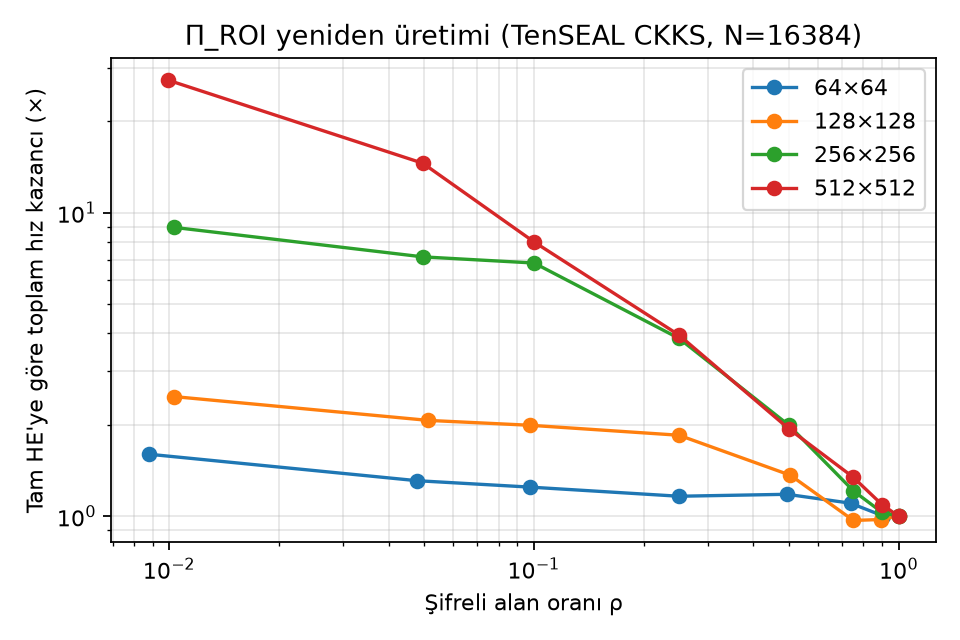
\includegraphics[width=12cm,keepaspectratio=true]{./fig/piroi_hiz_kazanci}
 \caption{Tam homomorfik şifrelemeye göre toplam hız kazancının şifreli alan oranı ve görüntü boyutuyla değişimi.}
 \label{fig:piroi}
\end{figure}

\section{Saldırı A: ROI Meta Verisinin Sızıntısı}\label{sec:res:A}

Çizelge \ref{tbl:saldiriA}, yalnızca protokolün serbest bıraktığı meta veriyi kullanan saldırının sonuçlarını göstermektedir.

\begin{table*}[h!]
{\setlength{\tabcolsep}{4pt}
\caption{Yalnızca ROI meta verisi ve girdi boyutuyla teşhis tahmini (AUC).}
\begin{center}
\vspace{-6mm}
\begin{tabular}{lllccc}
\hline\hline
Veri & Hedef & ROI & Öznitelikler & AUC & \%95 GA \\
\hline
Beyin MR & Tümör tipi (3 sınıf) & Tümör & Girdi boyutu & 0.457 & 0.401--0.519 \\
 & & & Konum & 0.775 & 0.743--0.804 \\
 & & & Büyüklük & 0.708 & 0.674--0.736 \\
 & & & Şekil & 0.722 & 0.691--0.747 \\
 & & & Tümü & 0.830 & 0.801--0.855 \\
\hline
COVID-QU-Ex & Teşhis (3 sınıf) & Akciğer & Konum & 0.729 & 0.720--0.739 \\
 & & & Büyüklük & 0.765 & 0.757--0.775 \\
 & & & Şekil & 0.780 & 0.771--0.788 \\
 & & & Tümü & 0.834 & 0.827--0.841 \\
 & Normal / pnömoni & Akciğer & Tümü & 0.904 & 0.895--0.913 \\
 & Normal / COVID-19 & Akciğer & Tümü & 0.853 & 0.842--0.863 \\
 & Pnömoni / COVID-19 & Akciğer & Tümü & 0.832 & 0.820--0.842 \\
 & COVID-19 / diğer & Enfeksiyon & ROI alanı & 1.000 & -- \\
\hline
Kaggle & Normal / pnömoni & -- & Girdi boyutu & 0.934 & -- \\
 & Normal / COVID-19 & -- & Girdi boyutu & 0.920 & -- \\
\hline
\end{tabular}
\vspace{-6mm}
\end{center}
\label{tbl:saldiriA}}
\end{table*}

Beyin MR verisinde tümörün konumu, büyüklüğü ve şekli birlikte tümör tipini makro AUC $0.830$ ile ele vermiştir. Sınıf bazında hipofiz tümörü AUC $0.949$, gliom $0.827$, meningiom $0.714$ ile ayırt edilmiştir. Permütasyon önemine göre en çok bilgi taşıyan öznitelik tümörün yatay ağırlık merkezidir (AUC düşüşü $0.102$). Bunu sınırlayıcı kutunun üst kenarı ($0.028$) ve kutu doluluğu ($0.023$) izlemiştir. Orta hatta yer alma, hipofiz tümörlerinin tipik konumuyla uyumludur. Bu veri kümesinde kesitlerin neredeyse tamamı aynı boyutta olduğundan girdi boyutu sızıntı yaratmamıştır (AUC $0.457$).

COVID-QU-Ex verisinde görüntülerin tamamı aynı çözünürlüğe getirildiği için yalnızca akciğer maskesinin geometrisi kullanılmıştır. Bu geometri teşhisi 3 sınıflı AUC $0.834$, normal ile pnömoni ayrımını AUC $0.904$ ile ele vermiştir. ROI'nin enfeksiyon maskesi olarak tanımlandığı uç durumda ROI alanı tek başına COVID-19 tanısını kusursuz biçimde ayırmıştır, çünkü enfeksiyonu olmayan görüntülerin ROI'si boştur. Orijinal çözünürlüklerin korunduğu Kaggle kümesinde ise ROI geometrisine hiç bakmadan yalnızca görüntü boyutu normal ile pnömoniyi AUC $0.934$ ile ayırmıştır.

\textbf{Kesit yönü kontrolü.} Çizelge \ref{tbl:yon}, beyin MR verisinde konum sızıntısının kesit yönünden kaynaklanıp kaynaklanmadığını sınayan kontrolün sonuçlarını vermektedir. Yalnızca kesit yönü tümör tipini neredeyse hiç ele vermemiştir (AUC $0.540$). Buna karşın meta veri saldırısı her yönün kendi içinde de güçlü kalmıştır. Yön tahmininin görsel olarak en güvenilir olduğu sagital grupta AUC $0.891$'dir (Şekil \ref{fig:yon}). Dolayısıyla meta veri sızıntısı kesit yönünün bir yan etkisi değildir.

\begin{table*}[h!]
{\setlength{\tabcolsep}{12pt}
\caption{Beyin MR verisinde kesit yönü kontrolü (tümör tipi, makro AUC).}
\begin{center}
\vspace{-6mm}
\begin{tabular}{lcc}
\hline\hline
Model girdisi & Kesit sayısı & AUC \\
\hline
Yalnızca kesit yönü & 3.064 & 0.540 \\
Yalnızca meta veri & 3.064 & 0.830 \\
Kesit yönü ve meta veri & 3.064 & 0.858 \\
Meta veri, yalnızca aksiyel kesitler & 1.126 & 0.841 \\
Meta veri, yalnızca koronal kesitler & 969 & 0.847 \\
Meta veri, yalnızca sagital kesitler & 969 & 0.891 \\
\hline
\end{tabular}
\vspace{-6mm}
\end{center}
\label{tbl:yon}}
\end{table*}

\begin{figure}[h!]
 \centering
 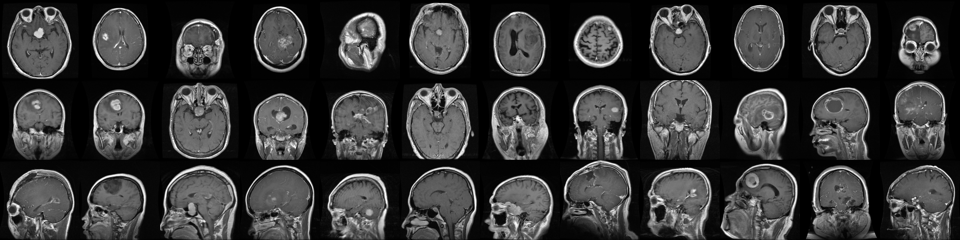
\includegraphics[width=15cm,keepaspectratio=true]{./fig/beyin_kesit_yonu_tahmini}
 \caption{Tahmin edilen kesit yönlerinden rastgele örnekler (satırlar: aksiyel, koronal, sagital). Görsel denetimde sagital grubun 12 örneğin 12'si, aksiyel grubun yaklaşık 9--10'u, koronal grubun yaklaşık 8'i doğru bulunmuştur.}
 \label{fig:yon}
\end{figure}

\section{Saldırı B: Açık Bağlamın Sızıntısı}\label{sec:res:B}

Çizelge \ref{tbl:saldiriB}, sunucunun gördüğü görüntüyle eğitilen CNN saldırganının sonuçlarını göstermektedir.

\begin{table*}[h!]
{\setlength{\tabcolsep}{6pt}
\caption{Bağlam saldırısında görüşe göre gizli alan oranı ve saldırgan AUC değeri.}
\begin{center}
\vspace{-6mm}
\begin{tabular}{lcccc}
\hline\hline
& \multicolumn{2}{c}{Beyin MR (tümör tipi)} & \multicolumn{2}{c}{COVID-QU-Ex (teşhis)} \\
Görüş & Gizli alan & AUC & Gizli alan & AUC \\
\hline
Tam (şifresiz) & 0.000 & 0.985 & 0.000 & 0.997 \\ % TOHUM: 5 tohum ortalamasiyla guncellenecek
Yalnız ROI & 0.983 & 0.979 & 0.765 & 0.990 \\
Bağlam ($\Pi_{\mathrm{ROI}}$ görüşü) & 0.017 & 0.976 & 0.235 & 0.993 \\ % TOHUM: guncellenecek
Bağlam + 10 piksel & 0.051 & 0.973 & 0.425 & 0.992 \\
Bağlam + 20 piksel & 0.101 & 0.968 & 0.609 & 0.989 \\
Bağlam + 40 piksel & 0.248 & 0.966 & 0.874 & 0.958 \\ % TOHUM: guncellenecek
ROI sınırlayıcı kutusu & 0.025 & 0.974 & 0.513 & 0.984 \\
\hline
\end{tabular}
\vspace{-6mm}
\end{center}
\label{tbl:saldiriB}}
\end{table*}

Her iki veri kümesinde de ROI'nin gizlenmesi saldırıyı neredeyse hiç zayıflatmamıştır. Beyin MR verisinde AUC $0.985$'ten $0.976$'ya, göğüs röntgeninde $0.997$'den $0.993$'e inmiştir. Göğüs röntgeninde akciğerler 40 piksel genişletilerek görüntünün \%87'si gizlendiğinde bile AUC $0.958$ kalmış, normal ile pnömoni ayrımı $0.951$ olmuştur. Yalnızca ROI'nin görüldüğü referans görüşte AUC değerlerinin ($0.979$ ve $0.990$) bağlam görüşüyle aynı düzeyde olması, ROI dışındaki bağlamın teşhis için ROI'nin kendisi kadar bilgi taşıdığını göstermektedir.

\section{Gerçekçilik Testi}\label{sec:res:transfer}

Kaggle görüntülerine akciğer maskesi üretmek için eğitilen U-Net, COVID-QU-Ex doğrulama bölmesinde Dice benzerliği $0.978$'e ulaşmıştır. Üretilen 6.432 maskenin hiçbirinde akciğer alanı görüntünün \%5'inden küçük çıkmamış, maskeler görsel denetimde de doğru bulunmuştur (Şekil \ref{fig:maske}). Tekrar eden görüntüler çıkarıldıktan sonra Kaggle kümesinde 340 normal ve 1.157 pnömoni görüntüsü kalmıştır. Çizelge \ref{tbl:transfer} kümeler arası sonuçları vermektedir.

\begin{table*}[h!]
{\setlength{\tabcolsep}{5pt}
\caption{Saldırganın farklı bir kaynaktan veriyle eğitildiği gerçekçilik testi (normal / pnömoni, AUC ve \%95 GA).}
\begin{center}
\vspace{-6mm}
\begin{tabular}{lcccc}
\hline\hline
Eğitim $\rightarrow$ test & Eğitim & Test & Tam görüntü & Akciğer gizli \\
\hline
COVID-QU-Ex $\rightarrow$ Kaggle & 17.571 & 1.497 & 0.999 (0.998--1.000) & 0.997 (0.995--0.999) \\
Kaggle $\rightarrow$ COVID-QU-Ex & 1.215 & 4.393 & 0.924 (0.916--0.932) & 0.938 (0.931--0.945) \\
COVID-QU-Ex $\rightarrow$ COVID-QU-Ex & 17.571 & 4.393 & 0.992 & 0.983 \\
\hline
\end{tabular}
\vspace{-6mm}
\end{center}
\label{tbl:transfer}}
\end{table*}

Hastanenin verisine hiç erişmeden, başka bir kaynaktan eğitilen saldırgan akciğerlerin şifreli olduğu görüntülerde pnömoniyi AUC $0.938$--$0.997$ ile bulmuştur. Küçük Kaggle kümesiyle eğitilen saldırganın akciğerler gizliyken daha iyi genellemesi ($0.924$'e karşı $0.938$), kaynaklar arasında taşınan bilginin önemli bölümünün akciğer dışında olduğuna işaret etmektedir. Kaggle kümesindeki normal ve pnömoni görüntüleri ile COVID-QU-Ex'in bir bölümü aynı çocuk hastalar kaynağından derlendiği için, bu test tamamen bağımsız bir hastane testi değildir (Bölüm \ref{sec:sinirliliklar}).

\begin{figure}[h!]
 \centering
 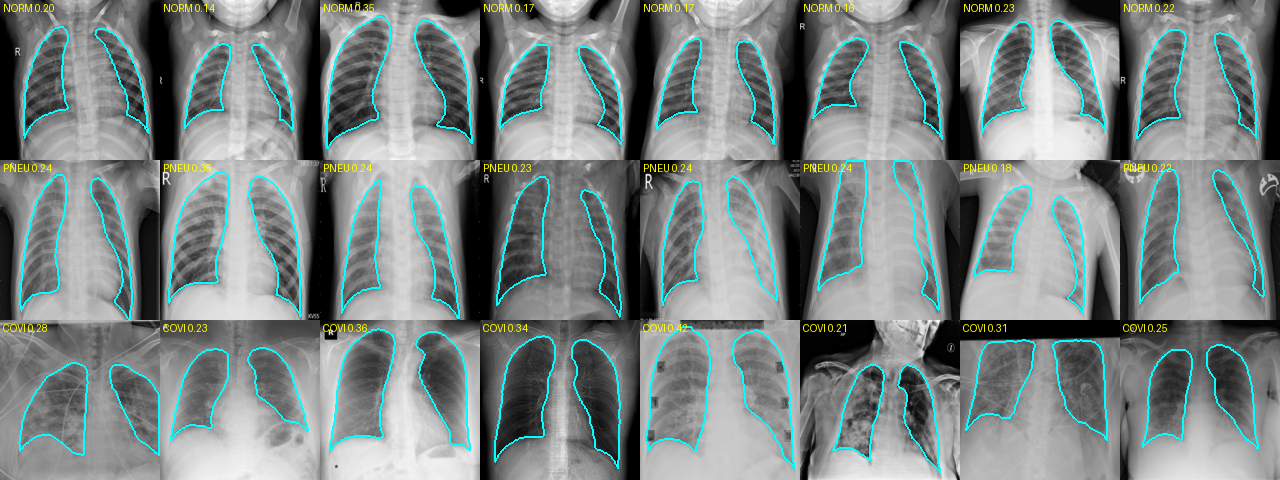
\includegraphics[width=15cm,keepaspectratio=true]{./fig/kaggle_akciger_maskeleri_kontrol}
 \caption{Kaggle göğüs röntgenlerine U-Net ile üretilen akciğer maskelerinden rastgele örnekler (satırlar: normal, pnömoni, COVID-19; sayı akciğer alanı oranıdır).}
 \label{fig:maske}
\end{figure}

\section{Sızıntının Kaynağı}\label{sec:res:root}

Çizelge \ref{tbl:gradcamcxr} ve Çizelge \ref{tbl:gradcambeyin}, bağlam görüşüyle eğitilen saldırganın Grad-CAM dikkat kütlesinin bölgelere dağılımını göstermektedir. Ortalama haritalar Şekil \ref{fig:camcxr} ve Şekil \ref{fig:cambeyin}'de verilmiştir.

\begin{table*}[h!]
{\setlength{\tabcolsep}{4pt}
\caption{Göğüs röntgeninde Grad-CAM dikkat kütlesinin bölgelere dağılımı.}
\begin{center}
\vspace{-6mm}
\begin{tabular}{lcccccc}
\hline\hline
Sınıf & Akciğer (gizli) & Kenar çerçeve & Akciğer üstü & Akciğer altı & Akciğerler arası & Yanlar \\
\hline
COVID-19 & 0.290 & 0.264 & 0.022 & 0.074 & 0.175 & 0.174 \\
Pnömoni & 0.255 & 0.270 & 0.032 & 0.057 & 0.186 & 0.198 \\
Normal & 0.280 & 0.262 & 0.042 & 0.049 & 0.222 & 0.144 \\
Tümü & 0.275 & 0.265 & 0.032 & 0.060 & 0.194 & 0.173 \\
\hline
\end{tabular}
\vspace{-6mm}
\end{center}
\label{tbl:gradcamcxr}}
\end{table*}

\begin{table*}[h!]
{\setlength{\tabcolsep}{10pt}
\caption{Beyin MR görüntüsünde Grad-CAM dikkat kütlesinin bölgelere dağılımı.}
\begin{center}
\vspace{-6mm}
\begin{tabular}{lcccc}
\hline\hline
Sınıf & Tümör (gizli) & Tümör çevresi & Beynin geri kalanı & Arka plan \\
\hline
Meningiom & 0.030 & 0.092 & 0.456 & 0.374 \\
Gliom & 0.033 & 0.103 & 0.433 & 0.431 \\
Hipofiz & 0.026 & 0.133 & 0.725 & 0.115 \\
Tümü & 0.030 & 0.109 & 0.525 & 0.323 \\
\hline
\end{tabular}
\vspace{-6mm}
\end{center}
\label{tbl:gradcambeyin}}
\end{table*}

Göğüs röntgeninde saldırganın dikkati akciğerin dışında geniş bir bağlama yayılmıştır: kenar çerçeve (\%27), kalp ve mediasteni içeren akciğerler arası bölge (\%19) ve göğüs yanları (\%17). Normal sınıfında akciğerler arası bölgenin payı daha yüksektir (\%22). Gizli akciğer bölgesinin de \%28 pay alması iki nedene bağlanmaktadır. Birincisi, son evrişim bloğundaki $7 \times 7$ çözünürlüklü haritanın büyütülürken sınırlardan taşmasıdır. İkincisi, saldırganın gösterge kanalı üzerinden akciğerin şeklini kullanabilmesidir. Beyin MR görüntüsünde dikkatin yarısı beynin geri kalanında, üçte biri kafa dışı arka plandadır. Gliom ve meningiom sınıflarında arka planın payının yüksek olması (\%37--43), görüntüleme alanına veya cihaza özgü izlerin de sızıntıya katkı sağladığına işaret etmektedir. Bu yorum Bölüm \ref{sec:res:defense}'daki savunma bulgusuyla da tutarlıdır: kafa dışında açık kalan 8 piksel bile tümör tipini ele vermektedir.

\begin{figure}[h!]
 \centering
 
\includegraphics[width=15cm,keepaspectratio=true]{./fig/kok_neden_gradcam_covidqu}
 \caption{COVID-QU-Ex verisinde akciğerler gizliyken saldırganın sınıf bazında ortalama Grad-CAM haritaları (camgöbeği çizgi ortalama akciğer sınırıdır).}
 \label{fig:camcxr}
\end{figure}

\begin{figure}[h!]
 \centering
 
\includegraphics[width=15cm,keepaspectratio=true]{./fig/kok_neden_gradcam_brain}
 \caption{Beyin MR verisinde tümör gizliyken saldırganın sınıf bazında ortalama Grad-CAM haritaları.}
 \label{fig:cambeyin}
\end{figure}

Çizelge \ref{tbl:onisleme}, önişleme adımlarının sızıntıya etkisini göstermektedir. Histogram eşitleme ve kenarın gizlenmesi saldırıyı anlamlı ölçüde zayıflatmamış, en güçlü birleşim bile AUC'yi yalnızca $0.993$'ten $0.988$'e indirmiştir. Sızıntı, basit önişlemeyle temizlenebilecek yüzeysel bir iz değildir.

\begin{table*}[h!]
{\setlength{\tabcolsep}{14pt}
\caption{COVID-QU-Ex verisinde önişleme adımlarının bağlam saldırısına etkisi (3 sınıf AUC).}
\begin{center}
\vspace{-6mm}
\begin{tabular}{lc}
\hline\hline
Önişleme & AUC \\
\hline
Yok & 0.993 \\
Histogram eşitleme & 0.993 \\
Dış kenarın \%5'inin gizlenmesi & 0.993 \\
Dış kenarın \%10'unun gizlenmesi & 0.991 \\
Histogram eşitleme ve \%10 kenar gizleme & 0.988 \\
\hline
\end{tabular}
\vspace{-6mm}
\end{center}
\label{tbl:onisleme}}
\end{table*}

\section{Savunmalar ve Gizlilik Şartlı Maliyet}\label{sec:res:defense}

Çizelge \ref{tbl:savunma}, savunma politikalarının seçilmiş noktalarını; Şekil \ref{fig:savcxr} ve Şekil \ref{fig:savbeyin} ise tüm eğrileri göstermektedir. Tamamen gizli kontrol görüşünde her iki veri kümesinde de AUC $0.500$ bulunmuş ve değerlendirme boru hattının doğru çalıştığı doğrulanmıştır.

\begin{table*}[h!]
{\setlength{\tabcolsep}{5pt}
\caption{Savunma politikalarında şifreli alan oranı, saldırgan AUC değeri ve protokol maliyetine göre hız kazancı.}
\begin{center}
\vspace{-6mm}
\begin{tabular}{llcccc}
\hline\hline
Veri & Politika & $\rho$ & AUC & Hız kazancı ($256^2$) & Hız kazancı ($512^2$) \\
\hline
COVID-QU-Ex & Varsayılan ROI (akciğer) & 0.234 & 0.990 & 4.04 & 4.17 \\
 & Kanonik ROI & 0.633 & 0.974 & 1.49 & 1.57 \\
 & Kanonik ROI + 16 piksel & 0.911 & 0.910 & 1.03 & 1.08 \\
 & Sızıntı-güdümlü, 4. adım & 0.827 & 0.919 & 1.11 & 1.20 \\
 & Sızıntı-güdümlü, 9. adım & 0.981 & 0.776 & 1.01 & 1.02 \\
 & Kanonik ROI + 32 piksel & 0.996 & 0.681 & 1.00 & 1.00 \\
 & Tamamen gizli (kontrol) & 1.000 & 0.500 & 1.00 & 1.00 \\
\hline
Beyin MR & Varsayılan ROI (tümör) & 0.016 & 0.941 & 8.65 & 24.24 \\
 & Kanonik ROI & 0.334 & 0.910 & 2.94 & 2.93 \\
 & Kanonik ROI + 32 piksel & 0.791 & 0.892 & 1.16 & 1.26 \\
 & Sızıntı-güdümlü, 10. adım & 0.884 & 0.842 & 1.05 & 1.11 \\
 & Sızıntı-güdümlü, 12. adım & 0.996 & 0.811 & 1.00 & 1.00 \\
 & Kanonik ROI + 64 piksel & 0.9998 & 0.619 & 1.00 & 1.00 \\
 & Tamamen gizli (kontrol) & 1.000 & 0.500 & 1.00 & 1.00 \\
\hline
\end{tabular}
\vspace{-6mm}
\end{center}
\label{tbl:savunma}}
\end{table*}

$\Pi_{\mathrm{ROI}}$'nin varsayılan kullanımında hız kazancı göğüs röntgeninde 4.2, beyin MR görüntüsünde 24 kattır; ancak teşhis neredeyse tamamen açıktadır (AUC $0.990$ ve $0.941$). Tüm görüntülerde aynı olan kanonik ROI, meta veri sızıntısını kapatsa da saldırıyı yalnızca $0.974$ ve $0.910$ düzeyine indirmiştir.

Saldırgan AUC'sini $0.8$'in altına indirmek için göğüs röntgeninde sızıntı-güdümlü politikanın 9. adımına, yani görüntünün \%98.1'inin şifrelenmesine (yalnızca 968 piksel açık) ihtiyaç duyulmuştur. Bu noktada $512 \times 512$ görüntüdeki hız kazancı 1.02 kattır. Beyin MR verisinde sızıntı-güdümlü politika \%99.6 şifreli alanda (226 piksel açık) bile $0.811$'de kalmış; $0.8$ hedefi ancak tam şifrelemeyle sağlanmıştır. $0.7$ ve $0.6$ hedefleri de pratikte yalnızca tam şifrelemeyle karşılanmıştır. Göğüs röntgeninde kanonik ROI + 32 piksel görüşü 190 açık piksel ile $0.681$'e inmiş, beyin MR verisinde ise kafa dışında açık kalan 8 piksel tümör tipini hâlâ AUC $0.619$ ile ele vermiştir.

Sızıntı-güdümlü seçim, göğüs röntgeninde aynı şifreli alanda rastgele yama seçiminden birkaç puan daha düşük AUC sağlamıştır; örneğin yaklaşık \%93 şifreli alanda $0.864$'e karşı $0.895$ ve $0.920$. Beyin MR verisinde ise iki politika arasında belirgin bir fark oluşmamıştır (yaklaşık \%94 şifreli alanda $0.859$'a karşı $0.858$ ve $0.862$). Savunma saldırganları hesaplama maliyetini sınırlamak için daha az veriyle eğitildiğinden, gerçek sızıntının bu değerlerden de yüksek olması beklenir.

\begin{figure}[h!]
 \centering
 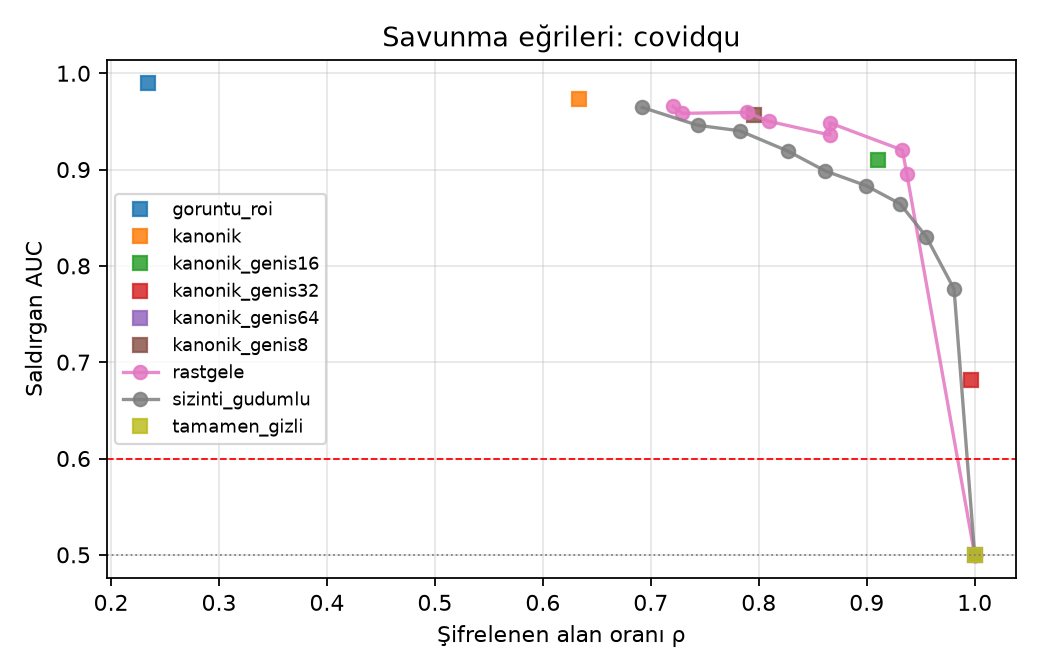
\includegraphics[width=12cm,keepaspectratio=true]{./fig/savunma_covidqu}
 \caption{COVID-QU-Ex verisinde savunma politikalarının şifreli alan oranına göre saldırgan AUC eğrileri (kırmızı kesikli çizgi $0.6$, gri noktalı çizgi şans düzeyidir).}
 \label{fig:savcxr}
\end{figure}

\begin{figure}[h!]
 \centering
 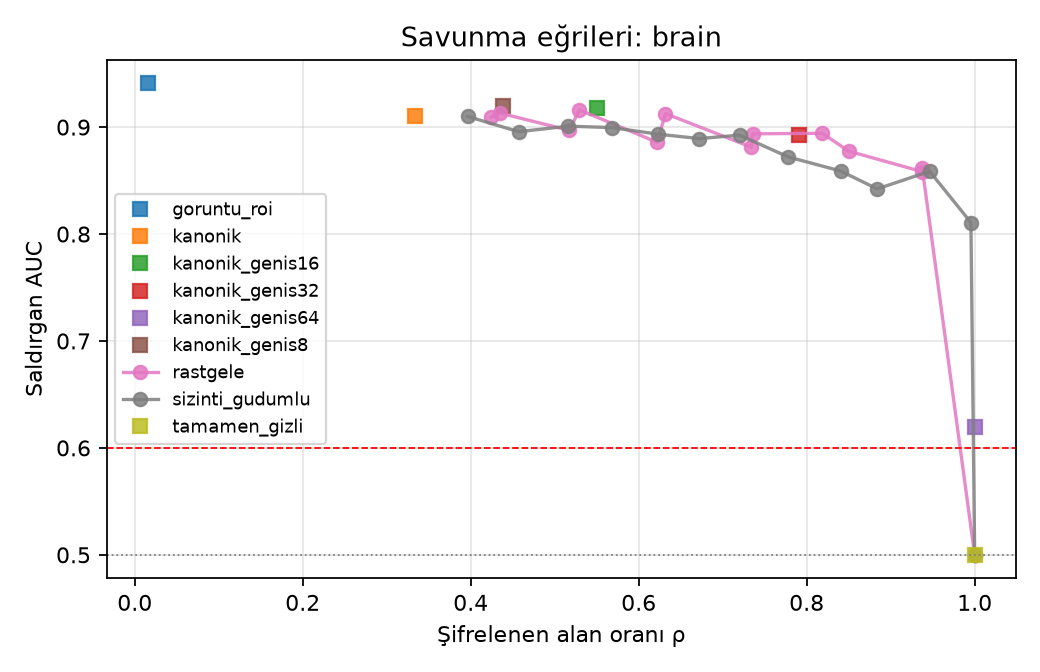
\includegraphics[width=12cm,keepaspectratio=true]{./fig/savunma_brain}
 \caption{Beyin MR verisinde savunma politikalarının şifreli alan oranına göre saldırgan AUC eğrileri.}
 \label{fig:savbeyin}
\end{figure}
